% This is "sig-alternate.tex" V2.1 April 2013
% This file should be compiled with V2.5 of "sig-alternate.cls" May 2012
%
% This example file demonstrates the use of the 'sig-alternate.cls'
% V2.5 LaTeX2e document class file. It is for those submitting
% articles to ACM Conference Proceedings WHO DO NOT WISH TO
% STRICTLY ADHERE TO THE SIGS (PUBS-BOARD-ENDORSED) STYLE.
% The 'sig-alternate.cls' file will produce a similar-looking,
% albeit, 'tighter' paper resulting in, invariably, fewer pages.
%
% ----------------------------------------------------------------------------------------------------------------
% This .tex file (and associated .cls V2.5) produces:
%       1) The Permission Statement
%       2) The Conference (location) Info information
%       3) The Copyright Line with ACM data
%       4) NO page numbers
%
% as against the acm_proc_article-sp.cls file which
% DOES NOT produce 1) thru' 3) above.
%
% Using 'sig-alternate.cls' you have control, however, from within
% the source .tex file, over both the CopyrightYear
% (defaulted to 200X) and the ACM Copyright Data
% (defaulted to X-XXXXX-XX-X/XX/XX).
% e.g.
% \CopyrightYear{2007} will cause 2007 to appear in the copyright line.
% \crdata{0-12345-67-8/90/12} will cause 0-12345-67-8/90/12 to appear in the copyright line.
%
% ---------------------------------------------------------------------------------------------------------------
% This .tex source is an example which *does* use
% the .bib file (from which the .bbl file % is produced).
% REMEMBER HOWEVER: After having produced the .bbl file,
% and prior to final submission, you *NEED* to 'insert'
% your .bbl file into your source .tex file so as to provide
% ONE 'self-contained' source file.
%
% ================= IF YOU HAVE QUESTIONS =======================
% Questions regarding the SIGS styles, SIGS policies and
% procedures, Conferences etc. should be sent to
% Adrienne Griscti (griscti@acm.org)
%
% Technical questions _only_ to
% Gerald Murray (murray@hq.acm.org)
% ===============================================================
%
% For tracking purposes - this is V2.0 - May 2012

\documentclass{sig-alternate-05-2015}
\usepackage{amsmath,epsfig}
\usepackage{graphicx}
\usepackage{caption}
\usepackage{algorithm}
\usepackage[noend]{algpseudocode}
\usepackage[center]{subfigure}
\usepackage{color,graphicx}
\usepackage{multirow}
\usepackage{cite}
\usepackage{textcomp}
\usepackage{amssymb}
\usepackage{algorithm}
\usepackage[noend]{algpseudocode}
\usepackage{listings}
\makeatletter
\def\BState{\State\hskip-\ALG@thistlm}
\makeatother
\begin{document}

% Copyright

%\setcopyright{acmlicensed}
%\setcopyright{rightsretained}
%\setcopyright{usgov}
%\setcopyright{usgovmixed}
%\setcopyright{cagov}
%\setcopyright{cagovmixed}
%
% --- Author Metadata here ---

%\CopyrightYear{2007} % Allows default copyright year (20XX) to be over-ridden - IF NEED BE.
%\crdata{0-12345-67-8/90/01}  % Allows default copyright data (0-89791-88-6/97/05) to be over-ridden - IF NEED BE.
% --- End of Author Metadata ---

\title{Can we refine the notion of what an acceptable ad is?}
\subtitle{}
%
% You need the command \numberofauthors to handle the 'placement
% and alignment' of the authors beneath the title.
%
% For aesthetic reasons, we recommend 'three authors at a time'
% i.e. three 'name/affiliation blocks' be placed beneath the title.
%
% NOTE: You are NOT restricted in how many 'rows' of
% "name/affiliations" may appear. We just ask that you restrict
% the number of 'columns' to three.
%
% Because of the available 'opening page real-estate'
% we ask you to refrain from putting more than six authors
% (two rows with three columns) beneath the article title.
% More than six makes the first-page appear very cluttered indeed.
%
% Use the \alignauthor commands to handle the names
% and affiliations for an 'aesthetic maximum' of six authors.
% Add names, affiliations, addresses for
% the seventh etc. author(s) as the argument for the
% \additionalauthors command.
% These 'additional authors' will be output/set for you
% without further effort on your part as the last section in
% the body of your article BEFORE References or any Appendices.

\numberofauthors{2} %  in this sample file, there are a *total*
% of EIGHT authors. SIX appear on the 'first-page' (for formatting
% reasons) and the remaining two appear in the \additionalauthors section.
%
\author{
% You can go ahead and credit any number of authors here,
% e.g. one 'row of three' or two rows (consisting of one row of three
% and a second row of one, two or three).
%
% The command \alignauthor (no curly braces needed) should
% precede each author name, affiliation/snail-mail address and
% e-mail address. Additionally, tag each line of
% affiliation/address with \affaddr, and tag the
% e-mail address with \email.
%
% 1st. author
\alignauthor
Arjun Gurumurthy\\
       \affaddr{Dept Of Computer Sciences}\\
       \affaddr{UW-Madison}\\
       \affaddr{Madison,Wisconsin}\\
       \email{arjun@cs.wisc.edu}
% 2nd. author
\alignauthor
Rogers Jeffrey\\
       \affaddr{Dept Of Computer Sciences}\\
       \affaddr{UW-Madison}\\
       \affaddr{Madison,Wisconsin}\\
       \email{rl@cs.wisc.edu}
}
\maketitle
\begin{abstract}
Ad blockers have caused an increasing amount of debate over the recent years, with the scope of arguments ranging from their economic impact to ethical considerations. A majority of ad blockers rely on whitelists and blacklists of websites to control the ads being displayed.
Adblock Plus, one of the widely used ad blockers, has enumerated a set of rules that an ad displaying page should follow for an advertisement to be determined as acceptable or not. In this project we investigate the behavior of adblock plus to  .Our study begins with the analysis of the ad-block plus filtering-mechanisms. Existing addons provide us with capability to understand the filtering process. We then analyze the behavior of adblock plus on 1500 webpages to see how adblock plus implements or enforces the acceptable ads criteria. We use our analysis to see if minor modifications to the page structure can cause the ads to pass through the filtering process of the adblocker. Our results show that adblock plus is too restrictive as it blocks non advertising related content. We also observe that adblock plus can be obviated by minor modifications to the web pages.
 \end{abstract}

%\terms{Theory}

\keywords{Ad Fraud,Impression Fraud,Acceptable Ads}

\section{Introduction}
Content and services which are offered for free on the Internet are sometimes monetized through online advertisements.
This relies on the implicit understanding that the viewers who consume free content do so at the cost of viewing ads.
However, recent times have seen the  rise of ad blockers that control the display of  advertisements on websites. These adblockers rely on  a list of filters for blocking or allowing advertisements.
In 2011 adblock plus started monetization of the whitelist by launching what is known was an "Acceptable ads" program.As a part of the acceptable ads program adblock plus proposed  that ads  displayed on a page have to adhere to. A publisher adhering to this crtieria can pay a fee to adblock plus and get themselves whitelisted. It is known that the e-commerce and advertising giants like Amazon, Google and Microsoft paid an undisclosed sum to adblock plus to get themselves whitelisted.

While the number of users of adblock plus continues to grow, on the other hand the number of filters added to the whitelist has also grown over the years.
<Insert fig>, indicates the growth of whitelist since 2011.
Unsurprisingly, one can see an increasing trend in the number of ads allowed by adblock plus.
This raises the following questions.
\begin{itemize}
\item [Q1.] How does whitelisting impact the number of ads blocked? \label{q:q1}
\item [Q2.] Does Adblock Plus allow ads even if they do not satisfy the criteria of an acceptable ad? \label{q:q2}
\item [Q3.] Does adblock Plus block ads even if they satisfy the four criteria?
\item [Q4.] As more sites are added to the whitelist when can adblock plus be deemed in-effective?
\end{itemize}
We attempt to answer Q1,Q2 and Q3 in our project by performing crawling web pages from different sources and analyzing the behavior of adblock plus on these webpages.


\section{Background}
Adblock plus is one of the widely use adblockers.
The Firefox add on alone has b403,191,426 downloads in total with 4,375,399 happening in the last 30 days ~\cite{abpmoz}.
Adblock plus relies  on filter lists for  its functioning.
The filter lists can be categorized into whitelists and blacklists.
The filters are nothing but text files that  have  a set of rules.
Blacklists contain rules for blocking advertisements whereas whitelists acts as exception for the rules that are in the blacklists.
The filters are  published and maintained by easylist~\cite{easylist}.
The rules in the white and blacklists are CSS and Xpath selectors that are prefixed with a predefined set of symbols.These rules interpreted as regular expressions by the adblock plus engine.
The notation is that filters prefixed with an $"@@"$ is a whitelisting filter and  filters prefixed with $"\#\#"$
or $\#@$  is  a blocking or blacklisting filter.
The blocking filters can be broadly classified into:
\begin{enumerate}
\item Element Hiding filters
\item URL filters
\end{enumerate}
Element hiding filters hide the elements present in an webpage from the user whereas the URL filters block the web page from requesting a resource , be it a webpage or javascript.

\section{{\secit Related Work}}
 General aspects of adblocking have been discussed in various studies. These studies have focussed on economic impact that adblockers have on advertising.  \cite{DigitalTrends} suggests that adblock railroads publishers and content providers to pay for their sites to be whitelisted.
<report> suggest that
in their report estimate the number of adblockusers at 2014 to be 144 million. They also
\cite{pujol2015annoyed} describe a method of classifying ad traffic by leveraging adblock plus. They use libadblock plus to classify the web traffic based on hits from the easylist and the whitelist. They also note that it is not possible to associate HTTP traffic with ad objects and that information is needed about the structure of the web page to achieve higher accuracy in detection of ad traffic. Finally, they establish that it is not possible to identify hidden ads without knowledge of the html page content.
By aiming to look at whether advertisements are acceptable or not, we are not just dealing with fraudulent ads that are propagated across the Internet, but also ads that a user would perceive as annoying or intrusive. In our process of understaning what an acceptable ad is, we look into existing definitions of what it means to be an acceptable advertisement.
\cite{walls2015measuring} describe criteria for an acceptable ad as defined by Adblock plus:
\begin{itemize}
\item Advertisements cannot contain animations, sounds, or "attention grabbing" images.
\item Advertisements cannot obscure page content or obstruct reading flow, i\.e\., the ad cannot be placed in the middle of a block
of text.
\item Advertisements must be clearly distinguished from the page
content and must be labeled using the word "advertisement"
or equivalent terms.
\item Banner advertisements should not force the user to scroll
down to view page content.
\cite{walls2015measuring} further present a comprehensive study of adblock plus and  an analysis of how the users perceive acceptable ads. They report that $ 90 \% $ of the users viewing an all grid layout ads could not distinguish them from the content. Allowing this ads thus seems to be in conflict with adblocks acceptable ads policies.
\end{itemize}

Furthermore , in their analysis of PPV networks \cite{springborn2013impression} describe a viewport size filter mechanism (a viewport is the user's visible area of a web page) for detecting ad views that are too small to be seen by the user.

It can be clearly seen that the html content of the web page has a ton of information that can be used to characterize the nature of the ad being displayed in the web page.
We thus concentrate our discussion on analysis of web page structure to detect and redefine unacceptable ads.

\section{Methodology}
We give an outline of the questions that we attempt to answer, and then elaborate:
\begin{itemize}
\item [Q1.] How to detect if an ad violates the current characteristics of an acceptable ad?
\item [Q2.] How do we classify if an ad is intrusive or not? \item [Q3.] Can an ad be annoying or intrusive even after satisying all these four criteria?
\item [Q4.] Also, based on classification of ads as annoying or intrusive, can we then detect some common patterns in the web pages that are deemed non-acceptable?
\item [Q5.] If so, can this be used to refine the notion of an acceptable ad?
\end{itemize}

Note that we term 'unacceptable' ads as ads that don't follow the criteria for acceptable ads as well as ads that could be considered annoying or intrusive even if they satisfy the 4 characteristics.
\begin{enumerate}
 \item One way to answer Q1 is to look at the working of existing ad blockers and see if they are able to perfectly predict whether an ad violates the current notions of acceptability.

 We start by looking at Adblock Plus - how does it deal with acceptable ads.
 All the current criteria for acceptable ads involve the page structure, and this implies that AdBlock Plus must have some way of analyzing the DOM structure of the web page content. Thus, a critical step is the analysis of the AdBlock Plus code. We then check if:

 (a) Does adblock Plus block ads even if they satisfy the four criteria?

 (b) Does Adblock Plus allow ads even if they do not satisfy the four criteria ?

 While ideally (a) or (b) should not happen, there might still be some exceptions. Such exceptions provide scope for improvement or refinement of the criteria used to identify acceptable ads.

 \item The next step is to obtain the data -  this can be done by crawling the pages that contain annoying or intrusive ads and then storing the web page contents, and the same for the pages without these ads. For obtaining the data, we crawl through the ad servers domain list that is obtainable from lists \cite{CommonCrawl} \cite{crussell2014madfraud} \cite{PeterLowe2013}
  A question arises here: How to obtain pages with only acceptable ads?
  For now, a simple way to look at acceptable ads is to consider that all ads blocked by the AdBlockPlus plugin as unacceptable, and the ones permitted through as acceptable. It needs to be thought of if there is a better approach.

\item We now have a set of pages ,some with acceptable ads and some without. We attempt to perform the following:
 \begin{enumerate}
 \item We then identify characteristics of acceptable ads or unacceptable ones - there are multiple ways to evaluate this: one to Looking at the DOM structure and identify if there are common patterns between ads that are acceptable, one to crowdsource and obtain users' subjective analysis of what constitutes an acceptable ad, the other is to try to have an image of pages with acceptable and unacceptable ones and see if they have some visual similarities, or match some aesthetic criteria. we go with analysis of the dom structure, as it is an objective measure.
 \item Given a new ad, can we then classify it as an acceptable or not? One way to do that is if we have a set of annoying and acceptable ads, given a new ad - can we classify it as acceptable or not. This looks to be a typical machine learning classification problem provided we identiy and specify the relevant features in the web page structure. This can be used to answer Q2.
 \end{enumerate}

 \item If possible, we check if we can refine the notion of an acceptable ad or not by the characteristics or modes of classification used in the previous step. That is, if we identify structural similarity with respect to acceptability, can this be exhibited as a further constraint to redefine what an acceptable ad is? This would help us answer Q3 - Q5.

 One example of a criteria to determine if an ad is acceptable or not: frequency of occurrence of the ad. If the same ad is loaded every time a set of pages is viewed, will it correlate with the ad being unacceptable?

 This whole process would have implications in ad fraud detection as well, as analysis of web pages would be helpful in determining ad fraud, assuming the correlation between unacceptable ads and fraudulent ads is not very low.
\end{enumerate}

\section{Data}
\begin{table}[]
\label{tab:website}
\begin{tabular}{|l|l|}
\hline
Domain         & Count of pages crawled \\ \hline
digitalspy     & 40                     \\ \hline
theguardian    & 40                     \\ \hline
variety        & 39                     \\ \hline
indiewire      & 23                     \\ \hline
hitfix         & 20                     \\ \hline
cinemablend    & 20                     \\ \hline
darkhorizons   & 20                     \\ \hline
empireonline   & 20                     \\ \hline
eonline        & 20                     \\ \hline
etonline       & 20                     \\ \hline
fandango       & 20                     \\ \hline
tmz            & 20                     \\ \hline
flickeringmyth & 20                     \\ \hline
goldderby      & 20                     \\ \hline
heyuguys       & 20                     \\ \hline
\end{tabular}
\centering
\caption{Top-15 Crawled Websites}
\end{table}

For our initial experiments on  undertanding the behavior of adblock we crawled webpages from  200 websites.
These websites were picked from the  top 500 websites as ranked by Alexa ~\cite{alexa} and included sites from the following domains: sports, shopping, news.

For measuring the impact of the whitelist and blacklist over time, we used the Wayback Machine from the Internet Archive ~\cite{wayback} to obtain the revisions of whitelist and blacklist from 2012 to 2016.
There were 72 revisions in total for the whitelist and 69 revisions for the blacklist. We obtained the whitelist and blacklist at the end of each year from 2012 to 2016.

To find the number of blocked elements for each filter combination, we required websites that had a relatively large number of ads.
This was needed to obtain a clear picture of the performance of AdBlock Plus on such ad-intensive pages.
The Newsdesk page of IMDB is a hub that links to many such websites. We crawled 1500 webpages from 130 websites.
Table ~\ref{tab:website} lists the top-15 websites and the webpage counts.

\section{Results}
\begin{figure}
	\centering
	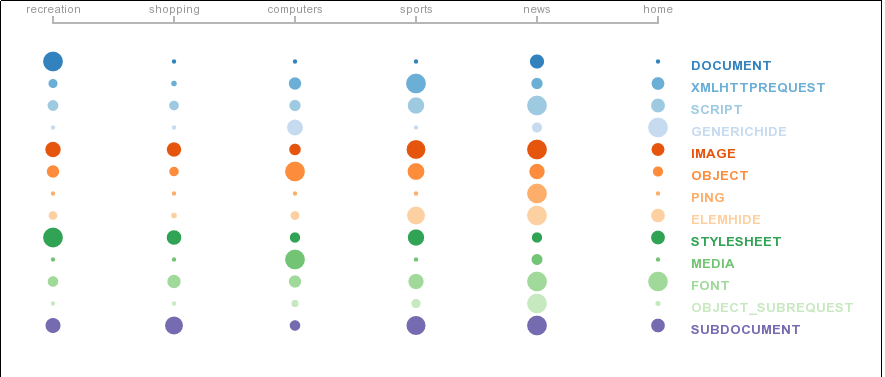
\epsfig{file=figures/abp_filters.png, width=0.50\textwidth}
	\vspace*{-0.5cm}
	\caption{\textbf{Filter Types in Adblock Plus}}
	\label{fig:abp-filters}
	\vspace*{-0.5cm}
\end{figure}
\begin{figure}
	\centering
	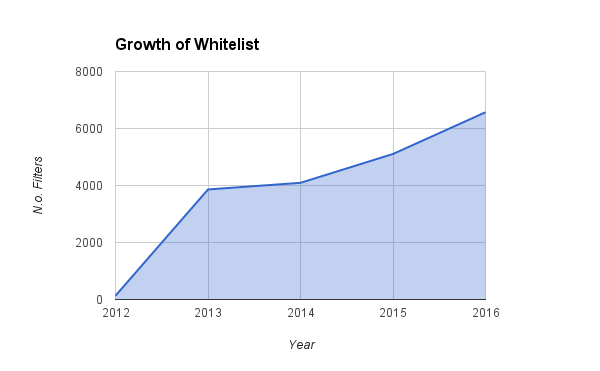
\epsfig{file=figures/growth.png, width=0.50\textwidth}
	\vspace*{-0.5cm}
	\caption{\textbf{Growth of Whitelist.}}
	\label{fig:growth}
	\vspace*{-0.5cm}
\end{figure}
\begin{figure}
Figure~\ref{fig:abp-filters} indicates the different types of filters  present in adblock.
The horizontal axis lists the domains associated with the webpages and the vertical axis lists the type of filter fired. The size of the circle corresponds to  the proportion of elements in that domain that are of a particular element type as indicated in the corresponding vertical axis. Looking at  particular domain from top to bottom shows the composition of various elements in the web pages belonging to that domain. In most of the cases  SCRIPT,IMAGE and SUBDOCUMENT can be seen as the dominating elements. These are the elements which the Adblock plus browser addon counts as an advertisement as a part of its statistics gathering.

Figure~\ref{fig:growth}, indicates the growth of whitelist since 2012. The aacceptable ads program had initially 132 filters in it. Over the years the whitelist has grown enormously in  size.  Over 3600 filters were added  between 2012 to 2013 and the list has been growing. As of March 2016, the total number of  filters in the whitelist is 6570.
Unsurprisingly, one can see an increasing trend in the number of ads allowed by adblock plus.
Figure~\ref{fig:ads-allowed}, shows the trend in the ads allowed over the years.

	\centering
	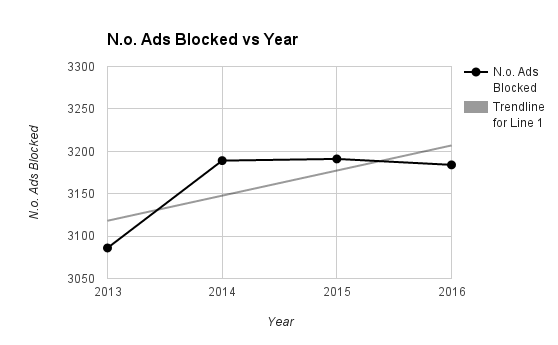
\epsfig{file=figures/alexa_ads.png, width=0.50\textwidth}
	\vspace*{-0.5cm}
	\caption{\textbf{Number of Ads allowed in the Alexa top 200.}}
	\label{fig:ads-allowed}
	\vspace*{-0.5cm}
\end{figure}

~\ref{fig:block-allow} shows the difference between the number of  elements  blocked  versus the number of elements allowed for three different  combuinations of the filters.
It can be seen that the list with only the element hiding filter does poorly in blocking the  elements as it does not have the capabilities of blocking URLS.
As expected the easylist+whitelist combination allows more ads there by allowing more elements.
\begin{figure}
	\centering
	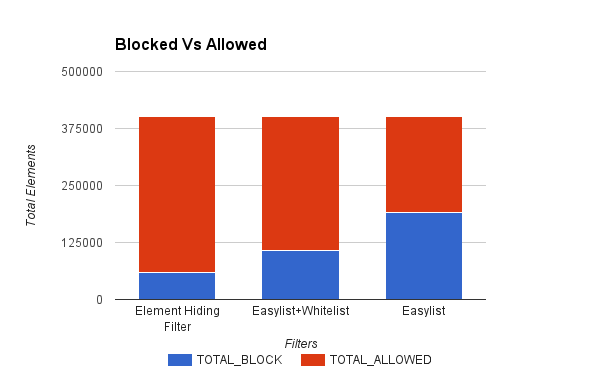
\epsfig{file=figures/exp_comparison.png, width=0.50\textwidth}
	\vspace*{-0.5cm}
	\caption{\textbf{Blocked vs Allowed for filter combinations}}
	\label{fig:block-allow}
	\vspace*{-0.5cm}
\end{figure}
\section{Conclusion and Future work}\label{sec:conclusions}
In our analysis, we observed that WideTable outperforms other views considered in the 
study.
The better performance was unaffected by the multiple memory configurations we tested 
in our analysis. 

A major takeaway in our analysis is that the cost of workload is affected significantly by 
the disk access patterns. 
Therefore the cost formulation should incorporate not just the buffer pool memory but 
also query characteristics such as types of joins, I/O access patterns, disk bandwidth etc. 
A sophisticated cost model involving the above parameters can help us in a more 
accurate modeling of the workload. 

We also feel that SSB is a simple benchmark which doesn't offer variety in terms of 
relational operations performed in the query. 
A complex benchmark like TPC-H should offer more challenges in analysis. 

Lastly, the LP formulation should allow selection of multiple views, instead of one view 
per workload, as it is assumed right now. 
This will allow us to choose the best view for a given query and potentially maximizing 
the performance gain for the workload. 
It will also make the LP not so obvious, unlike the current LP which can be solved using a 
simple greedy algorithm.

%\end{document}  % This is where a 'short' article might terminate
% The following two commands are all you need in the
% initial runs of your .tex file to
% produce the bibliography for the citations in your paper.
\bibliographystyle{abbrv}
\bibliography{sigproc}  % sigproc.bib is the name of the Bibliography in this case
% You must have a proper ".bib" file
%  and remember to run:
% latex bibtex latex latex
% to resolve all references
%
% ACM needs 'a single self-contained file'!
%

\end{document}
